%%%%%%%%%%%%%%%%%%%%%%%%%%%%%%%%%%%%%%%%%%%%%%%%%%%%%%%%%%%%%%%%%%%%%%
% Problem statement
\begin{statement}[
  problempoints=100,
  timelimit=3 sekunde,
  memorylimit=512 MiB,
]{Sadnice}

Krajem ožujka 2018. godine, gospodin Malnar se s lokalnog
obiteljsko-poljoprivrednog gospodarstva vratio s hrpom ljutih paprika.
S lakoćom ih je povezao špagama na optimalan način te ih, sasvim nesebično,
podijelio skupini prijatelja. Prvi ih je kušao Dominik koji nije ni osjetio
ljutinu, potom Josip i tako dalje. Međutim, dio prijatelja gospodina Malnara
ozbiljno se opekao. Među njima valja istaknuti Krešimira, koji se zakleo da
će mu se osvetiti.

Danas gospodin Malnar više ne kupuje paprike, već ih sam uzgaja. Ove godine
odlučio je posaditi $(N+1) \cdot (M+1)$ sadnica u koordinatnom sustavu, i to
tako da se sadnice nalaze na cjelobrojnim točkama iz skupa $\{0,1,2,\dots,N\}
\times \{0,1,2,\dots,M\}$. Također, odlučio je sadnice međusobno povezati
koristeći $(N+1)(M+1)-1$ komad špage jedinične duljine, odnosno, dvije
sadnice može direktno povezati komadom špage ako euklidska udaljenost između
njih iznosi $1$. Dodatno, sadnice moraju biti tako povezane da čine jedan
\textit{vijenac}. Za dvije sadnice kažemo da dio istoga vijenca ako sićušni
mravac, koji se kreće isključivo sadnicama i špagama, može proputovati između
spomenute dvije sadnice.

\begin{figure}[H]
  \begin{center}
    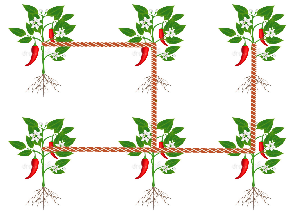
\includegraphics[width=0.4\textwidth]{img/skica.png}
    \caption*{Primjer ispravnog povezivanja sadnica za $N=1$ i $M=2$.}
  \end{center}
\end{figure}
  \vspace{-0.7cm}

Gospodin Malnar zna da mu Krešimir želi pomrsiti planove. Naslutio je da će
doći, pod okriljem noći, te napraviti točno jedan horizontalan ili
vertikalan rez kojim će prerezati svaki komad špage koji mu se nađe na putu.
Poznato je da Krešimir neće nauditi samim sadnicama, ali će njegov rez biti
takav da se početni vijenac sadnica raspadne na što je moguće više vijenaca.

Stoga, gospodin Malnar će povezati sadnice na način da broj vijenaca nakon
Krešimirova reza bude najmanji mogući.

Možete li odrediti jedan način na koji je gospodin Malnar mogao povezati
svoje sadnice?

%%%%%%%%%%%%%%%%%%%%%%%%%%%%%%%%%%%%%%%%%%%%%%%%%%%%%%%%%%%%%%%%%%%%%%
% Input
\subsection*{Ulazni podaci}
U prvom su retku prirodni brojevi $N$ i $M$ iz teksta zadatka.

%%%%%%%%%%%%%%%%%%%%%%%%%%%%%%%%%%%%%%%%%%%%%%%%%%%%%%%%%%%%%%%%%%%%%%
% Output
\subsection*{Izlazni podaci}
Potrebno je ispisati $2N+1$ redaka s po $3M+1$ znakova koji predstavljaju
na koji su način sadnice povezane komadima špage.

Sadnice predstavljamo znakom \texttt{'o'} (ASCII $111$), komad špage kojim
spajamo dvije sadnice u istom stupcu predstavljamo znakom \texttt{'|'} (ASCII
$124$), a komad špage kojim spajamo dvije sadnice u istom retku predstavljamo
znakovima \texttt{'-{}-'}.

Između susjednih sadnica koje nisu spojene komadom
špage nalaze se bjeline, i to dva znaka razmaka (ASCII $32$) između sadnica u
istom retku, odnosno znak za novi redak \texttt{'\textbackslash{}n'} (ASCII $10$)
između sadnica u istom stupcu.

%%%%%%%%%%%%%%%%%%%%%%%%%%%%%%%%%%%%%%%%%%%%%%%%%%%%%%%%%%%%%%%%%%%%%%
% Scoring
\subsection*{Bodovanje}
Rješenja koja na nekom test podatku na ispravan, ali ne i optimalan način
povežu sadnice, osvojit će $\frac{3}{4}(1 - \sqrt{1 - \frac{A^3}{B^3}})$
bodova, pri čemu $A$ označava broj vijenaca nakon Krešimirova reza u optimalnom
rješenju, dok $B$ označava analognu stvar u vašem rješenju.

Broj bodova nekog podzadatka jednak je najmanjem broju bodova koje vaše rješenje
ostvaruje na nekom od test podataka tog podzadatka.

{\renewcommand{\arraystretch}{1.4}
  \setlength{\tabcolsep}{6pt}
  \begin{tabular}{ccl}
 Podzadatak & Broj bodova & Ograničenja \\ \midrule
  1 & 15 & $1 \le N = M \le 1\,000$ \\
  2 & 15 & $2 \le 2N = M \le 1\,000$ \\
  3 & 10 & $1 \le N \le M \le 3$ \\
  4 & 20 & $1 \le N \le M \le 10$ \\
  5 & 20 & $1 \le N \le M \le 100$ \\
  6 & 20 & $1 \le N \le M \le 1\,000$ \\
\end{tabular}}

%%%%%%%%%%%%%%%%%%%%%%%%%%%%%%%%%%%%%%%%%%%%%%%%%%%%%%%%%%%%%%%%%%%%%%
% Examples
\subsection*{Probni primjeri}
\begin{tabularx}{\textwidth}{X'X}
\sampleinputs{test/sadnice.dummy.in.1}{test/sadnice.dummy.out.1} &
\sampleinputs{test/sadnice.dummy.in.2}{test/sadnice.dummy.out.2}
\end{tabularx}


%%%%%%%%%%%%%%%%%%%%%%%%%%%%%%%%%%%%%%%%%%%%%%%%%%%%%%%%%%%%%%%%%%%%%%
% We're done
\end{statement}

%%% Local Variables:
%%% mode: latex
%%% mode: flyspell
%%% ispell-local-dictionary: "croatian"
%%% TeX-master: "../hio.tex"
%%% End:
